\appendix
%\addcontentsline{toc}{section}{Appendices}
\section{Appendices}
\pagenumbering{roman}
\subsection{Stewart Platform and Wind Tunnel Configurations}
\includepdf[pages=-]{Wind Tunnel Assembly + Stewart}
\includepdf[pages=-]{Assemby 3 2}
\clearpage
\subsection{Budget and TimePlan}
\subsubsection{Provisional Budget}
\begin{center}
	\begin{table}[H]
		\centering
		\caption{Proposed budget}
		\paragraph{ }
		\includegraphics{Figures/budget}
	\end{table}
\end{center}
\subsubsection{Work Plan}
\begin{center}
	\begin{table}[H]
		\centering
		\caption[Time plan]{Time plan for first and second semester}
		\paragraph{ }
		\includegraphics[width=0.95\linewidth]{Figures/workplan}
	\end{table}
\end{center}
\clearpage
\subsection{Production Plan}
\includepdf[pages=-]{Production plan}

\clearpage

\subsection{Force transformation matrix}
In such a case the forces experienced at the top of the platform are distributed between the 6 legs and as result, a force transformation matrix is required to resolve the forces applied on each axis as measured by each load cell on each leg.

If the platform is acted upon by an external wrench {$\vec{F}_e, \vec{M}_e$}, for static equilibrium of the body, the external wrench is statically balanced by the six leg forces of the Stewart platform. Representing the unit vector $\hat{I}_i$ along the i-th leg with respect to B, the leg force is given  by $\hat{I}_if_i$. Considering the force equilibrium of the platform along  three mutually perpendicular directions in B(XYZ), the following force equations can be obtained as in \cite{dwarakanath_design_2001}:

\begin{ceqn}
	\begin{align}
		(F_e)_x = f_1I_{1x} + f_2I_{2x} + f_3I_{3x} + f_4I_{4x} + f_5I_{5x} + f_6I_{6x}
	\end{align}
\end{ceqn}
\begin{ceqn}
	\begin{align}
		(F_e)_y = f_1I_{1y} + f_2I_{2y} + f_3I_{3y} + f_4I_{4y} + f_5I_{5y} + f_6I_{6y}
	\end{align}
\end{ceqn}
\begin{ceqn}
	\begin{align}
		(F_e)_z = f_1I_{1z} + f_2I_{2z} + f_3I_{3z} + f_4I_{4z} + f_5I_{5z} + f_6I_{6z}
	\end{align}
\end{ceqn}
where $(F_e)_x$, $(F_e)_y$ and $(F_e)_z$ are the external forces on the platform along three mutually perpendicular directions x, y and z of the frame B, respectively.

The moment due to the forces $\hat{I}_if_i$ about the origin of B is $(\vec{b}_i x \hat{I}_i)f_i$. Considering the moment equilibrium about x, y and z axes of B, the following moment equations can be obtained as in \cite{dwarakanath_design_2001}:

\begin{ceqn}
	\begin{align}
		(M_e)_x = f_1(\vec{b}_1 x \hat{I}_1)_x + f_2(\vec{b}_2 x \hat{I}_2)_x + f_3(\vec{b}_3 x \hat{I}_3)_x + f_4(\vec{b}_4 x \hat{I}_4)_x + f_5(\vec{b}_5 x \hat{I}_5)_x + f_6(\vec{b}_6 x \hat{I}_6)_x
	\end{align}
\end{ceqn}
\begin{ceqn}
	\begin{align}
		(M_e)_y = f_1(\vec{b}_1 x \hat{I}_1)_y + f_2(\vec{b}_2 x \hat{I}_2)_y + f_3(\vec{b}_3 x \hat{I}_3)_y + f_4(\vec{b}_4 x \hat{I}_4)_y + f_5(\vec{b}_5 x \hat{I}_5)_y + f_6(\vec{b}_6 x \hat{I}_6)_y
	\end{align}
\end{ceqn}
\begin{ceqn}
	\begin{align}
		(M_e)_z = f_1(\vec{b}_1 x \hat{I}_1)_z + f_2(\vec{b}_2 x \hat{I}_2)_z + f_3(\vec{b}_3 x \hat{I}_3)_z + f_4(\vec{b}_4 x \hat{I}_4)_z + f_5(\vec{b}_5 x \hat{I}_5)_z + f_6(\vec{b}_6 x \hat{I}_6)_z
	\end{align}
\end{ceqn}

where $(M_e)_x$, $(M_e)_y$ and $(M_e)_z$ are the external moments on the platform  about the three coordinate axes of B. Combining the equations the relationship between the external wrench and the forces experienced by the legs can be expressed as follows:
\begin{ceqn}
	\begin{align}
		\begin{Bmatrix}
			\vec{F}_e \\
			\vec{M}_e \\
		\end{Bmatrix} = [H]\{F\}
	\end{align}
\end{ceqn}
\clearpage
\subsection{Code}
The complete firmware and HMI programs can be found in this repository,

https://github.com/SammyOina/stewart-platform.
\clearpage

\subsection{PCB schematics}
\subsubsection{schematics}
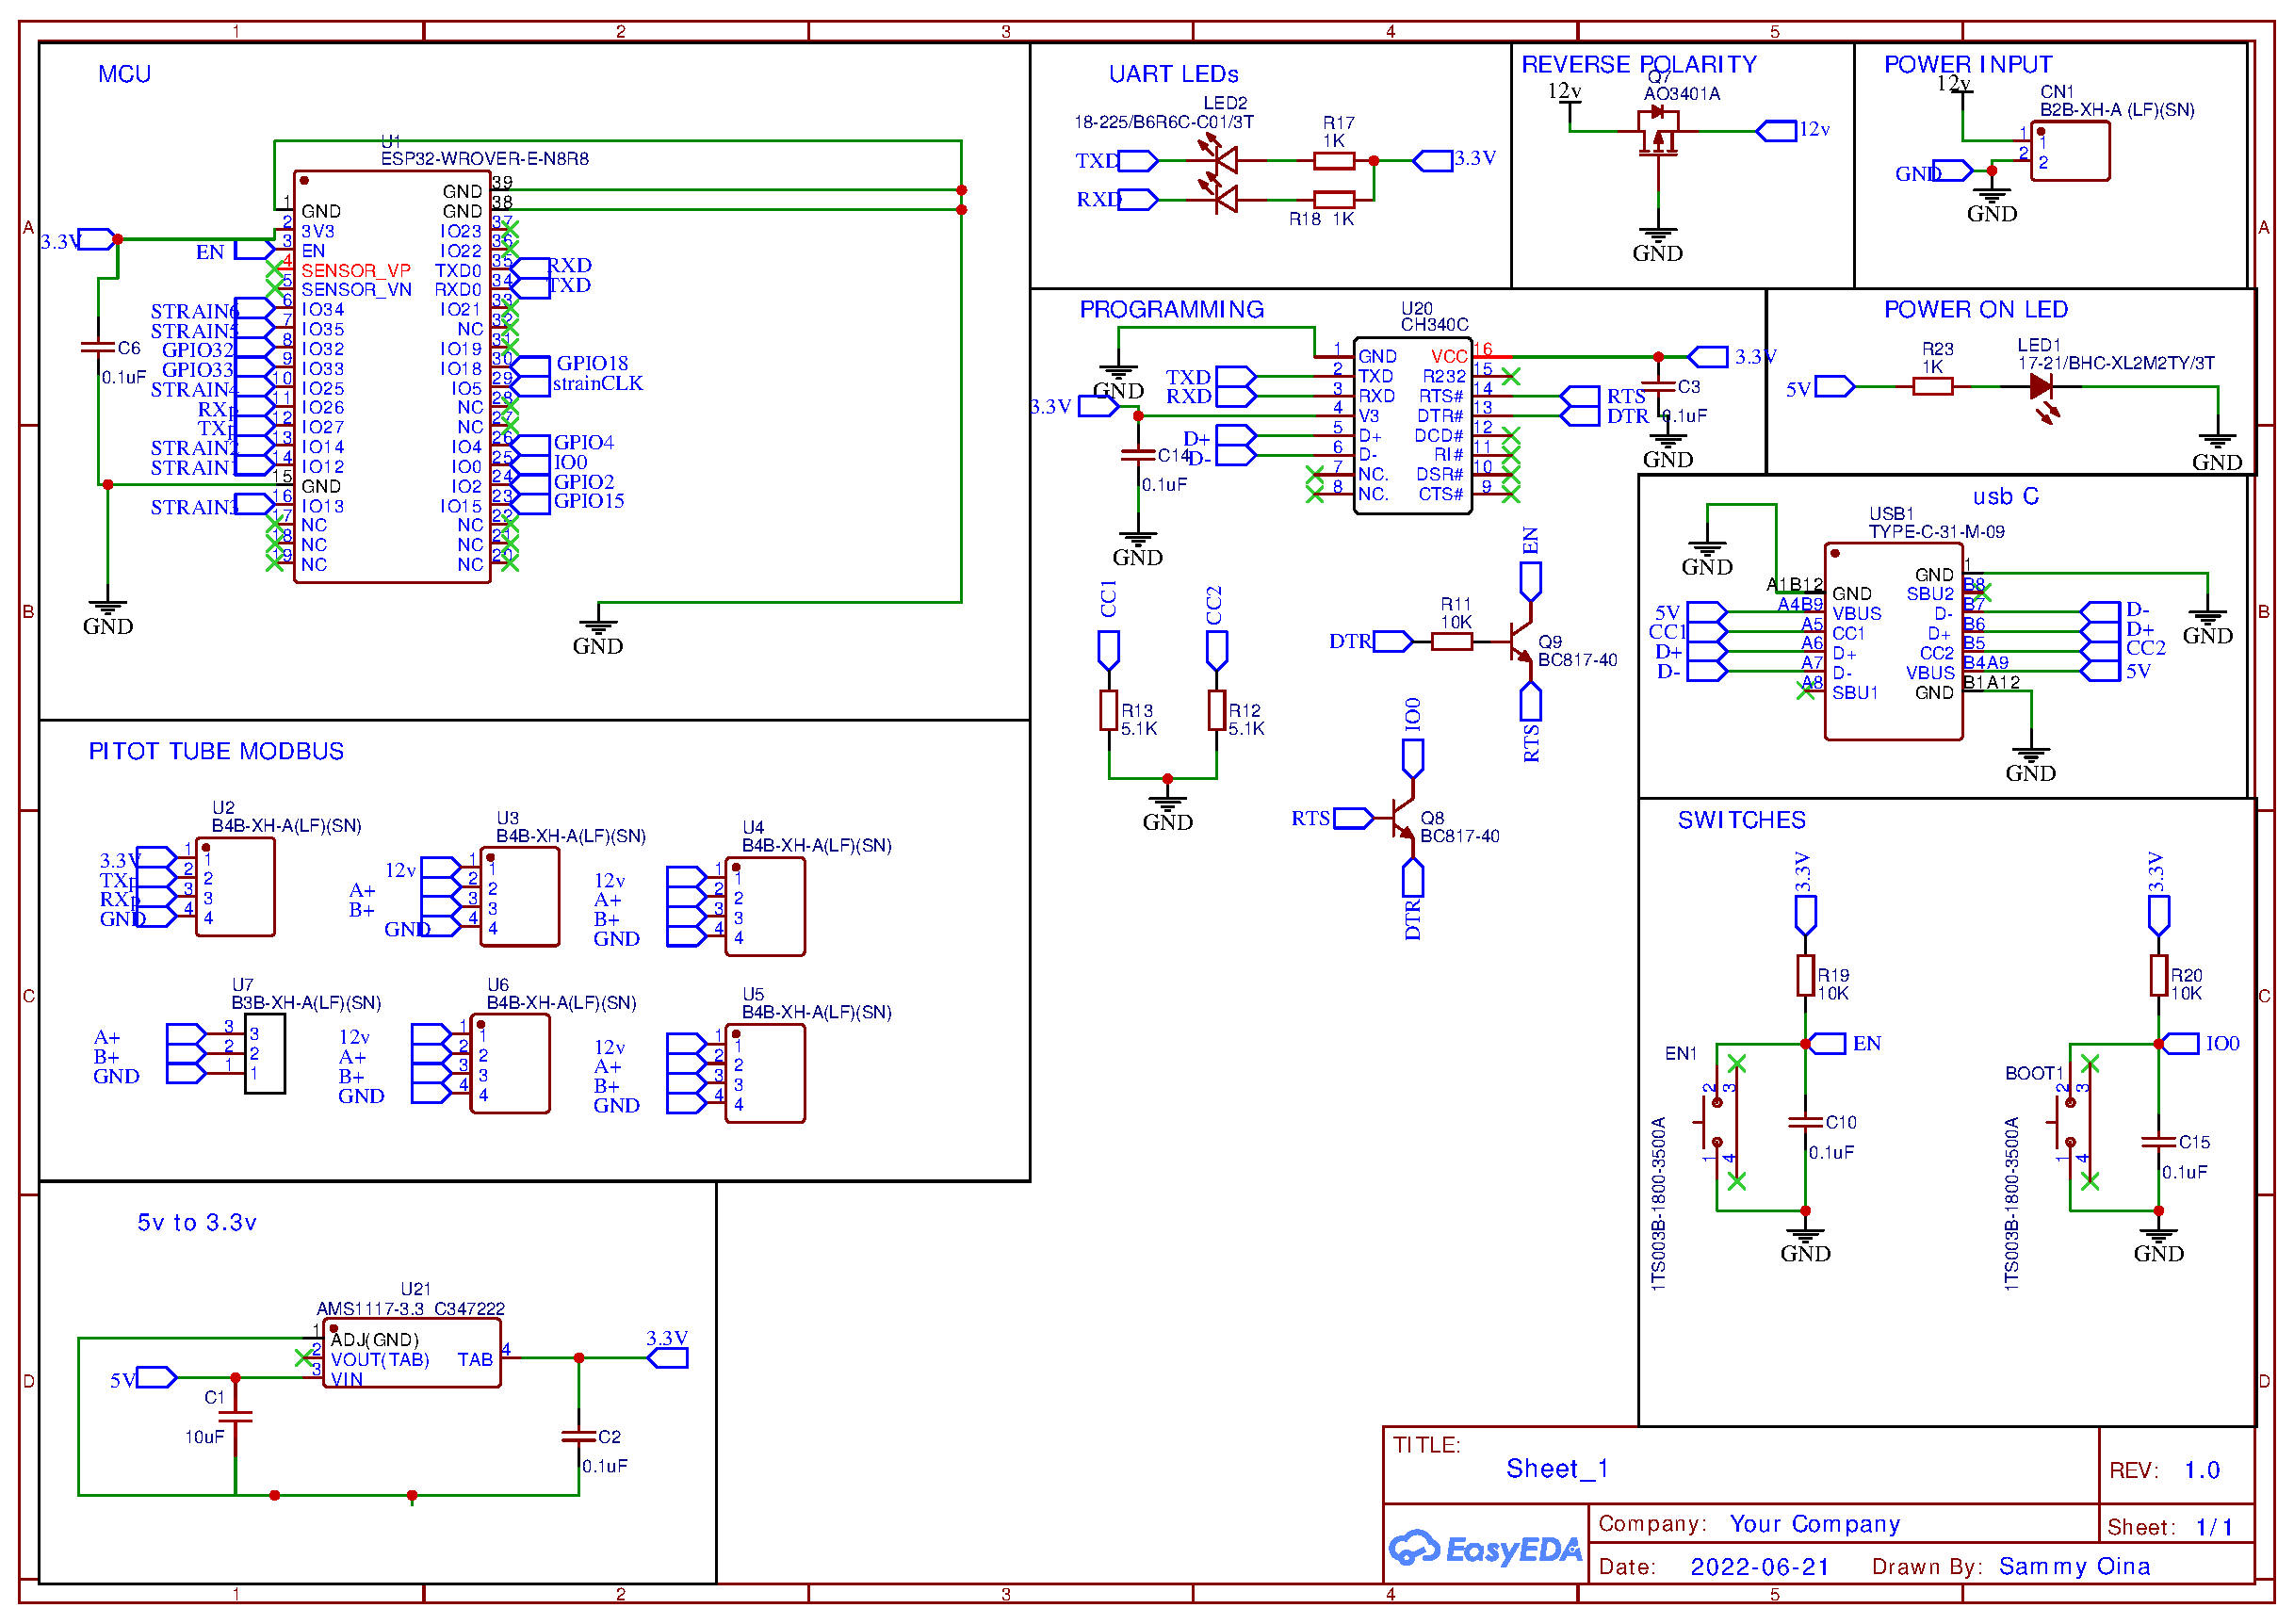
\includepdf[pages=-]{Figures/schm}